%; whizzy paragraph -pdf xpdf -latex ./whizzypdfptex.sh
%; whizzy-paragraph "^\\\\begin{frame}"
% latex beamer presentation.
% platex, latex-beamer でコンパイルすることを想定。 

%     Tokyo Debian Meeting resources
%     Copyright (C) 2009 Junichi Uekawa
%     Copyright (C) 2009 Nobuhiro Iwamatsu

%     This program is free software; you can redistribute it and/or modify
%     it under the terms of the GNU General Public License as published by
%     the Free Software Foundation; either version 2 of the License, or
%     (at your option) any later version.

%     This program is distributed in the hope that it will be useful,
%     but WITHOUT ANY WARRANTY; without even the implied warranty of
%     MERCHANTABILITY or FITNESS FOR A PARTICULAR PURPOSE.  See the
%     GNU General Public License for more details.

%     You should have received a copy of the GNU General Public License
%     along with this program; if not, write to the Free Software
%     Foundation, Inc., 51 Franklin St, Fifth Floor, Boston, MA  02110-1301 USA

\documentclass[cjk,dvipdfmx,12pt]{beamer}
\usetheme{Tokyo}
\usepackage{monthlypresentation}
%  preview (shell-command (concat "evince " (replace-regexp-in-string "tex$" "pdf"(buffer-file-name)) "&"))
%  presentation (shell-command (concat "xpdf -fullscreen " (replace-regexp-in-string "tex$" "pdf"(buffer-file-name)) "&"))
%  presentation (shell-command (concat "evince " (replace-regexp-in-string "tex$" "pdf"(buffer-file-name)) "&"))

%http://www.naney.org/diki/dk/hyperref.html
%日本語EUC系環境の時
\AtBeginDvi{\special{pdf:tounicode EUC-UCS2}}
%シフトJIS系環境の時
%\AtBeginDvi{\special{pdf:tounicode 90ms-RKSJ-UCS2}}

\title{東京エリア Debian 勉強会}
\subtitle{資料}
\author{岩松 信洋 iwamatsu@debian.or.jp\\IRC nick: iwamatsu}
\date{2009年12月12日}
\logo{
\includegraphics[width=8cm]{image200607/openlogo-light.eps}}

\begin{document}

\frame{\titlepage{}}

\emtext{設営準備にご協力ください}

\section{}
\begin{frame}
 \frametitle{Agenda}
\begin{minipage}[t]{0.45\hsize}
  \begin{itemize}
  \item 注意事項
	\begin{itemize}
	 \item 飲食可能
	\end{itemize}
  \item 最近あったDebian関連のイベント報告
	\begin{itemize}
	 \item 前回の勉強会
	 \item Adam C Powell IV 来日
	 \item Dirk Eddelbuettel 来日
	\end{itemize}
 \end{itemize}
\end{minipage} 
\begin{minipage}[t]{0.45\hsize}
 \begin{itemize}
  \item 一年の勉強会を振り返る
  \item 2009年、2010年、2011年
  \item qemubuilder
  \item lxc
  \item BSP, BSP, BSP
 \end{itemize}
\end{minipage}
\end{frame}


\begin{frame}
 \frametitle{2009年11月}
\begin{minipage}[t]{0.45\hsize}
  \begin{itemize}
  \item 注意事項
	\begin{itemize}
	 \item 飲食禁止
	\end{itemize}
  \item 最近あったDebian関連のイベント報告
	\begin{itemize}
	 \item 前回の勉強会
	\end{itemize}
 \end{itemize}
\end{minipage} 
\begin{minipage}[t]{0.45\hsize}
 \begin{itemize}
  \item Debian Quiz
  \item Debian ではじめる数学事始め
  \item Debian autobuilder
 \end{itemize}
\end{minipage}
\end{frame}

\begin{frame}{Dirk Eddelbuettel}
 写真ない? 
\end{frame}

\begin{frame}{Adam C Powell IV}

 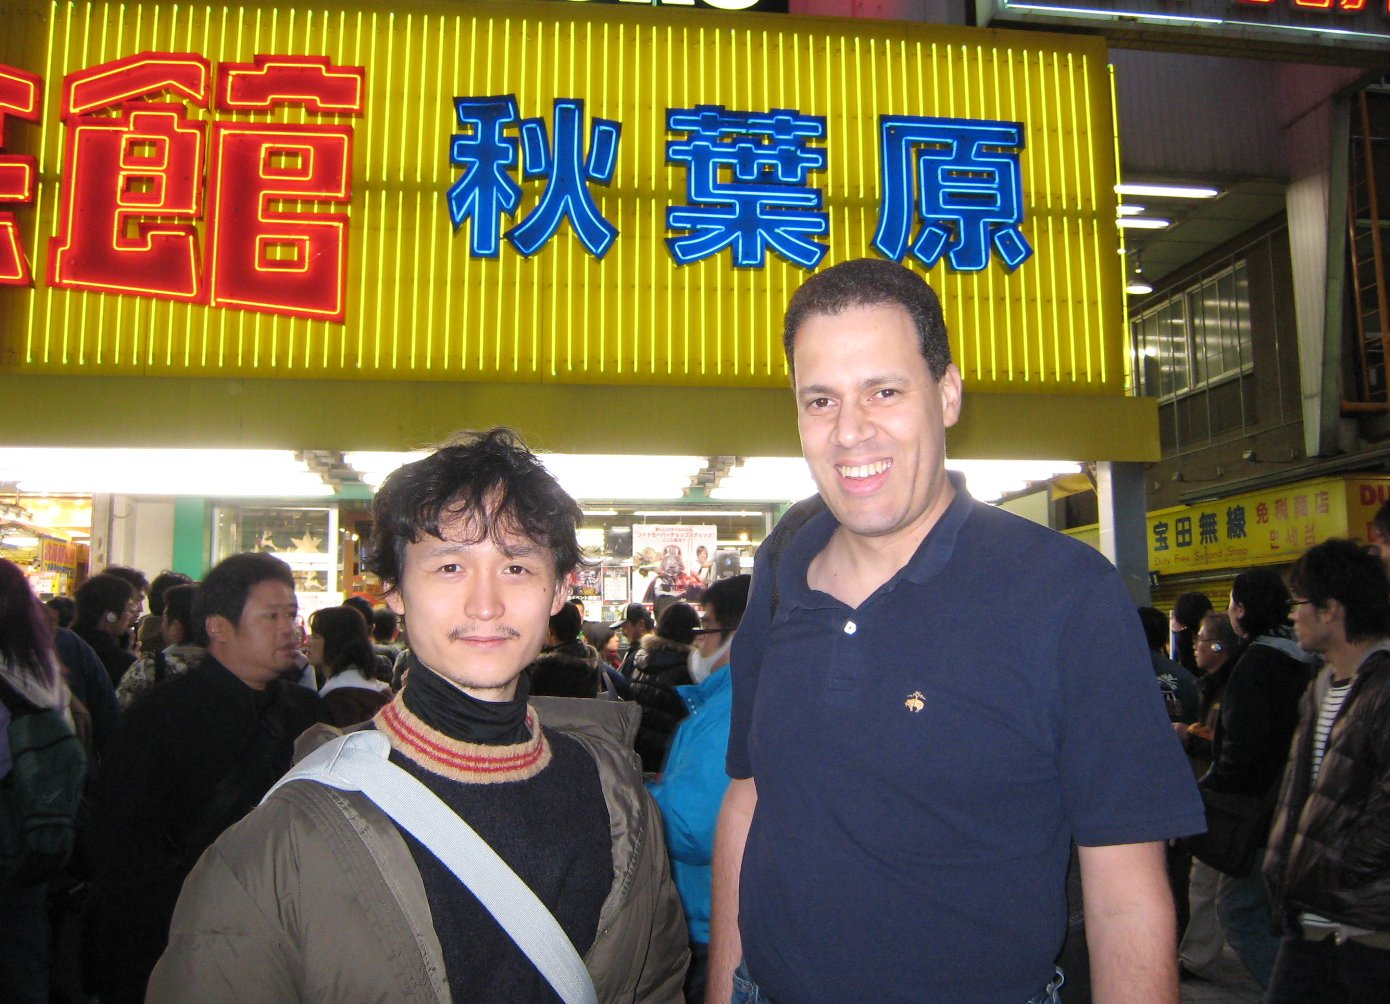
\includegraphics[width=1\hsize]{image200912/acp.jpg}

\end{frame}

\begin{frame}{Hack Cafe}

毎週水曜日、週に一回東京のどっかのカフェでハック。\\
\url{http://twitter.com/debian_hackcafe}\\
関西でも始めたようです。
\end{frame}

\begin{frame}{2009年計画}

{\scriptsize
 \begin{enumerate}
  \item 新年の企画 (アンサンブル荻窪開催)
  \item OSC Tokyo
  \item VAIO P インストール記録、
	カーネル読書会 ディストリビューション大集合(小林さん)(東京大学?)
  \item Git Handson (岩松)(あんさんぶる荻窪?)
  \item 家Debianサーバ vs 職場のネットワーク(千代田区都立図書館?\footnote{\url{http://www.library.chiyoda.tokyo.jp/}})
  \item DDTSS 
  \item スペインにて開催
  \item Debconf報告会
  \item Asterisk (東京大学?)、udev + HAL
  \item OSC Fall? (10月30・31日)
  \item 3D graphics 開発 
  \item Debian サーバ+VMware + 各種OS、
	他の仮想化ツール(vserver etc.)、
	忘年会
 \end{enumerate}
}
\end{frame}

\emtext{事前課題}

\begin{frame}{事前課題}
\begin{enumerate}
 \item 2009年を振り返って自分は何をしたか
 \item 2009年を振り返ってDebian関連で世間では何が起こったか
\end{enumerate}
\end{frame}

{\footnotesize
%; whizzy-master ../debianmeetingresume200912.tex
% $B0J>e$N@_Dj$r$7$F$$$k$?$a!"$3$N%U%!%$%k$G(B M-x whizzytex $B$9$k$H!"(Bwhizzytex$B$,MxMQ$G$-$^$9!#(B

\begin{prework}{$B>e@n=c0l(B}
\preworksection{2009$BG/$r?6$jJV$C$F<+J,$O2?$r$7$?$+(B}

2009$BG/!"H>J,$/$i$$$7$+(BDebian$BJY6/2q$K$O;22C$7$F$^$;$s!#(B

DDTSS $B$r$3$=$3$=$d$C$F$^$7$?$,!"5$$E$$$?$i:#G/$O(BDDTSS$B$N%5!<%P$,$H$^$C$?(B
 $B$j$H$$$m$$$m$H5/$-$?$h$&$G$9!#(B
%$BDI5-$9$k(B

\preworksection{2009$BG/$r?6$jJV$C$F(BDebian$B4XO"$G@$4V$G$O2?$,5/$3$C$?$+(B}

Netwalker $B$,%j%j!<%9$5$l$^$7$?$M!#(B
%$BDI5-$9$k(B

\end{prework}

\begin{prework}{$B5HED=SJe(B}
\preworksection{2009$BG/$r?6$jJV$C$F<+J,$O2?$r$7$?$+(B}
Debian$B4X78$@$H(BDDTSS$B$G%l%S%e!<$rCf?4$K(B180$B7oDxEY$d$C$F$$$?$h$&$G$9!#(B
DDTSS$B$O5Y$s$@$j$d$C$?$j!"$^$C$?$j$d$C$F$$$^$9!#(B
$B%$%Y%s%H4XO"$G$O(B2$B7n$K(BLinux conf.au$B$K9T$C$F!"=)$O(BJLS$B$K%\%i%s%F%#%";22C!"(B
KOF$B$K9T$C$F4X@>(BDebian$B$NJ}$H%-!<%5%$%s$r$7$?$j$7$F$$$^$7$?!#(B
$B$"$H$ONcG/DL$j!)$"$s$I$-$e$a$s$F$C$I$G$S$"$s$N%4!<%9%H%(%G%#%?!<7sGd$j;R$H$7$F!"(B
$BK?=j$GJY6/2q;qNA$r$^$H$a$FK\$K$7$FHRI[$7$F$$$^$9!#(B
\preworksection{2009$BG/$r?6$jJV$C$F(BDebian$B4XO"$G@$4V$G$O2?$,5/$3$C$?$+(B}
$B$d$O$j(BLenny$B%j%j!<%9$,0lHV$G$7$g$&!#(B
$B4pK\E*$K(Bstable$B$r;H$&%A%-%s$J$N$G!"%a%8%c!<%P!<%8%g%s%"%C%W$OBg$-$J(B
$B%K%e!<%9$G$9!#(B
$B:G6a$N(BDebian$B$ODj4|E*$K%j%j!<%9$5$l$k$N$G3F<o%=%U%H$b%P!<%8%g%s$,(B
$B3d$H?7$7$/!"JXMx$K46$8$F$$$^$9!#(B
$B$*$+$2$G;H$$$?$$%=%U%H$N$?$a$K!"(Bsid$BEy$+$i%P%C%/%]!<%H$7$?$j!"(B
$B$=$N$[$+(Btar$B%\!<%k$+$i%S%k%I$9$kI,MWEy$b>/$J$/$J$j!"$^$?$=$N>l9g$N<j4V$b(B
$B@N(B(woddy$B$N:"(B)$B$KHf$Y$F$+$J$j8:$C$F$*$j$"$j$,$?$$$G$9!#(B
\end{prework}

\begin{prework}{$B$^$($@$3$&$X$$(B}
\preworksection{2009$BG/$r?6$jJV$C$F<+J,$O2?$r$7$?$+(B}

$B%h%a$K(B Debian (Sid)$B$r;H$o$;;O$a$?!"(BHack Cafe, Debian JP Project $B$NA*5s4I(B
 $BM}0Q0w!"(BDebian $BJY6/2q$N1?1D$d!"$O$8$a$F$N(B ITP, DebConf9 $B;22C!"$O$8$a$F(B
 $B$N<9I.Ey!"$A$g$3$A$g$3$d$C$F$-$^$7$?$,!"$d$m$&$H;W$C$F$$$?$3$H$O$J$+$J(B
 $B$+$G$-$F$$$J$$$N$,8=>u$G$9!#(B(ITP$B$7$CJ|$7$K$7$F$7$^$C$F$$$k$7!D!#(B)

$BMhG/$O!"$b$&$9$3$7%^%k%A%?%9%/$G!JMWNNNI$/!KF0$1$k$h$&$K$7$?$$!"$H$$$&$+(B
$B$7$J$$$H$$$+$s$J$!$H;W$&G/$N@%$G$7$?!#(B

\preworksection{2009$BG/$r?6$jJV$C$F(BDebian$B4XO"$G@$4V$G$O2?$,5/$3$C$?$+(B}

OpenBlockS 600 $B$,=P$^$7$?$M!#(BOpenBlockS 266 $B$[$ILLGr$_$O$J$$$G$9$,!"%9%Z%C(B
 $B%/$,>e$,$C$F$b>CHqEENO$,Dc$$(B(5W)$B$N$ONI$$$G$9$M!#(B
\end{prework}

\begin{prework}{$B$d$^$M$R$G$-(B}
\preworksection{2009$BG/$r?6$jJV$C$F<+J,$O2?$r$7$?$+(B}
$B0J2<$G4v$D$+$N9`L\$KJ,$1$F?6$jJV$C$F$_$^$9!#(B

\subsubsection{$B%Q%C%1!<%8$N:n@.$H0];}(B}
$B<g$K%U%)%s%H$N%Q%C%1!<%8$K$D$$$FDI2C$r<B;\$7$^$7$?!#0J2<$,DI2C$5$l$?%Q%C%1!<%8$G$9!#(B

\begin{itemize}
 \item ttf-umefont - $B!VG_%U%)%s%H!W$N%Q%C%1!<%8$G$9(B
 \item ttf-umeplus - PCLinuxOS$B$NI8=`%U%)%s%H(B umeplus $B$N%Q%C%1!<%8$G$9!#(B
 \item ttf-ipafont/ttf-ipafont-jisx0208/otf-ipafont - IPA$B%U%)%s%H$G$9!#(B
 \item ttf-monapo - mona$B%U%)%s%H$H(BIPA$B%U%)%s%H$N9g@.%U%)%s%H$G$9(B
 \item ttf-sawarabi-gothic -$B!V$5$o$i$S%4%7%C%/!W%U%)%s%H$G$9!#(B
 \item ttf-misaki - $B!VH~:i%U%)%s%H!W$G$9!#(B
 \item ttf-kanjistrokeorders -$B!V4A;z$N=q$-=g!W%U%)%s%H$G$9!#F|K\8l3X=,<T$K?M5$$G$9!#(B
\end{itemize}

$B$"$H$O(B ITP $B$7$?$^$^:n6H$,;_$^$C$F$$$?$j(B reject $B$5$l$F:FD4@0$,$G$-$F$$$J$$$N$,4v$D$+$"$j$^$9$N$G!"(B
$B$=$l$rJRIU$1$F$$$1$l$P$H;W$$$^$9!#(B

\subsubsection{$BK]Lu:n6H(B}
$B%&%'%V$K$D$$$F$O!"(BDevelopers News $B$N::FI$dK]Lu:n6H!"$=$l$+$i(B po-debconf $B$N99?7$H?75,K]Lu:n6H$r<B;\$7$F$$$^$9!#(B
$B;DG0$J$,$i(B i18n.debian.net $B%5!<%P$,@5>o$K2TF/$7$F$$$J$$$N$G!"(Bpo-debconf $B$N?JD=>u67$O:rG/$HHf$Y$F$I$NDxEY>e$,$C$F$$$k$N$+$OITL@$G$9$,!"8eB`$O$7$F$$$J$$$O$:$G$9!J8=>u$G(B 70\% $B0J>e$O:n6H$7$F$$$k!K!#(B

$B$"$H$O(B upstream $B$G2?$+$G$-$l$P!"$H;W$$!"$3$3?tF|$G$O$"$k$b$N$N(B GNOME $B$NK]Lu99?7:n6H$K<j$r=P$7$F$_$F$$$^$9!#(B
2.30 $B%j%j!<%9$N:"(B (2010/3 $B$+$J!)(B) $B$K92$F$:$K::FI$^$G$G$-$l$PNI$$$G$9$M!#(B

\subsubsection{$B%$%Y%s%H!?9-Js7O$J3hF0(B}
Debian/Ubuntu$B3hF04XO"$G5-;v$r>/$7=q$+$;$F$$$?$@$$$?$j!"BPCL$K;22C$5$;$F$b$i$C$?$j$7$F$$$^$7$?!#(B

\begin{itemize}
 \item Software Design 2009/07 $BFC=8!V=i?4<T$K$d$5$7$/!$%Y%F%i%s$bK~B-!*!V(BDebian GNU/Linux 5.0$B!J(BLenny$B!K$r$*4+$a$9$kM}M3!W(B
 \item Software Design 2009/10 $B!V(BDebian GNU/Linux$B%+%s%U%!%l%s%9!V(BDebconf9$B!W<h:`%l%]!<%H(B Debian$B3+H/<T$,=8$&%9%Z%$%s(B14$BF|4V!W(B
 \item ThinkIT$B!V(BTOMOYO Linux$BE0Dl2rK6!!Bh(B3$B2s!'(BDebian$B$G(BTOMOYO Linux$B$r;H$&!W(B
 \item ascii.jp$B!V9T$C$H$1!*(BUbuntu$BF;>l!W(B
 \item $B%"%9%-!<%a%G%#%"%o!<%/%9!V=54)%"%9%-!<JL:}(B $B$5$/$5$/(BUbuntu!$B!W(B
\end{itemize}

$B$^$?!"%$%Y%s%H$K4v$D$+;22C$7$^$7$?!#:#G/$OBND4$,0-$+$C$?$3$H$b$"$j!":rG/$h$j>/$J$a$G$9(B (KOF$B$H$+9T$1$J$+$C$?!D(B)

\begin{itemize}
 \item Linux Consortium 10 Years Event !!$B!V%*!<%W%s%=!<%9%G%9%/%H%C%W$NL$Mh!W(B(2009/01)
 \item $BBh(B17$B2s%*!<%W%s%=!<%9%F%/%N%m%8!<JY6/2q!w(BGREE Labs$B!J(B2009/04$B!K(B
 \item Ubuntu 9.04 $B%*%U%i%$%s%_!<%F%#%s%0(B (2009/04)
 \item Open Source Conference Tokyo/Fall (2009/11)
\end{itemize}

$B>e5-$NCf$G!"<B<AE*$KH/I=$7$?$N$O(B GREE Labs $B$@$1$G$7$?$N$G!"MhG/$O$b$&>/$7BND4$r@0$($F!"%M%?$r$+$^$;$l$P!"$H;W$$$^$9!#(B


\subsubsection{Debconf9 $B;22C(B}
$B$h$&$d$/(B Debconf $B$K;22C$9$k$3$H$,$G$-$^$7$?!#$,!"$H$j$"$($:9T$C$?$@$1$G=*$o$C$F$k$N$G!"(B
$B$b$&>/$7<B@S$r@Q$`$3$H$H1Q8l$G$N%3%_%e%K%1!<%7%g%s$r2~A1$G$-$l$P$H;W$C$F$$$^$9!#(B

\preworksection{2009$BG/$r?6$jJV$C$F(BDebian$B4XO"$G@$4V$G$O2?$,5/$3$C$?$+(B}
$B$&!<$s!"@$4V$H$$$&$H$=$s$J$K%$%s%Q%/%H$OM?$($i$l$F$$$J$$$+$J!<$H8D?ME*$K$O46$8$F$$$^$9!#(B
\end{prework}

\begin{prework}{$BK\>190E5(B}
\preworksection{2009$BG/$r?6$jJV$C$F<+J,$O2?$r$7$?$+(B}

$B;E;v$,K;$7$/JY6/2q$b7g@J$7$,$A$G$7$?!#(B
$BL@F|$+$i4hD%$k!#(B

\preworksection{2009$BG/$r?6$jJV$C$F(BDebian$B4XO"$G@$4V$G$O2?$,5/$3$C$?$+(B}

SmartQ5$B$,=P$^$7$?!#(B
\end{prework}

\begin{prework}{$B%-%?%O%i(B}
\preworksection{2009$BG/$r?6$jJV$C$F<+J,$O2?$r$7$?$+(B}

$BD>@\(B Debian $B$G$J$/?=$7Lu$J$$$N$G$9$,!&!&!&!#(B
$B$3$N=)!"<B2H$K(B ADSL $B0z$-$^$7$F!"(B Ubuntu $B%$%s%9%H!<%k$7$?%N!<%H(B PC $B$r(B
$BCV$$$F$-$^$7$?!#!!%M%C%H%5!<%U%#%s@lMQ5!$G$9$,!"F@$KJ86g$b$J$/IaDL$K(B
$B;H$C$F$$$k$h$&$G$9!#!!(Bdebian $B7O(B linux $B%f!<%6$r0l?MA}$d$7$?$H$$$&$3$H$G!#(B

\preworksection{2009$BG/$r?6$jJV$C$F(BDebian$B4XO"$G@$4V$G$O2?$,5/$3$C$?$+(B}

$BF17oB??t$+$bCN$l$^$;$s$,!"(B Lenny $B%j%j!<%9$G$9$+$M!#(B
$B@$4V$X$N%$%s%Q%/%H$O!&!&!&!";d$N$^$o$j$G$O$"$^$j$J$+$C$?$h$&$J!)!*(B
\end{prework}

\begin{prework}{$BF|HfLn(B $B7<(B}
\preworksection{2009$BG/$r?6$jJV$C$F<+J,$O2?$r$7$?$+(B}

\begin{itemize}

\item Debian$BJY6/2q$G(BC$B$d(BPerl$B0J30$N8@8l$K$bCmL\$7$F$b$i$*$&$H!"(BOCaml$B$d(BCommon Lisp$B$NI[653hF0$r$7$^$7$?!#(B
\item Debian$BJY6/2q$G(BCommon Lisp$B%M%?$NH/I=$r$7$^$7$?!#(B

\end{itemize}

\preworksection{2009$BG/$r?6$jJV$C$F(BDebian$B4XO"$G@$4V$G$O2?$,5/$3$C$?$+(B}

\begin{itemize}

\item lenny$B%j%j!<%9!#2q<R$N%^%7%s$b%"%C%W%G!<%H$,I,MW$K$J$C$FBgJQK;$7$+$C$?!#(B
\item Debian$BJY6/2q$N1c2q$G$N%h%?OC$b$-$C$+$1$N0l$D$K$J$C$F!"F|K\$G$O=i$N(BOCaml$BFC2=%$%Y%s%H!"(B OCaml Meeting Tokyo 2009$B$G3+:E!#$_$J$5$s$K46<U!#(B

\end{itemize}

\end{prework}

\begin{prework}{$B4d>>(B $B?.MN(B}
\preworksection{2009$BG/$r?6$jJV$C$F<+J,$O2?$r$7$?$+(B}
\begin{itemize}
\item Debian Developer$B$K$J$C$?!#(B\\
Debian Developer$B$K$J$C$?$N$G!"%9%]%s%5!<$r9T$&$h$&$K$7$?!#(B
$B$$$^$^$G$d$C$F$b$i$C$?$3$H$r$d$k$h$&$K?4$,$1$k$h$&$K$7$F$$$k!#(B

\item Debian JP Project Leader $B$K$J$C$?!#(B
$B$J$<$+(B DJPL $B$J$C$F$$$k!#(B

\item Debian SH4 Port $BI|3h(B\\
Debconf9$B$K$$$C$F(B $BB>$N(BPorter$B$H:n6H$,$G$-$?$N$,Bg$-$$!#(B
$B$3$N@.2LJ*$rMxMQ$7$?@=IJ$b=P$?$h$&$G$9!#(B

\item $B;R6!$,@8$^$l$?(B
$B;R6!$,@8$^$l$?$N$G!"@83h$,0lJQ$7$?!#(B

\end{itemize}

\preworksection{2009$BG/$r?6$jJV$C$F(BDebian$B4XO"$G@$4V$G$O2?$,5/$3$C$?$+(B}
\begin{itemize}
\item Lenny $B$,%j%j!<%9$5$l$?(B
\item GPG$B80(B 4096R $B$X$N0\9T(B
\item glibc $B$+$i(B eglibc $B$X$N0\9T(B
\end{itemize}

\end{prework}

}

\emtext{Debian常識クイズ}

\section{DWN quiz}
\begin{frame}{Debian 常識クイズ}

Debian の常識、もちろん知ってますよね?
知らないなんて恥ずかしくて、知らないとは言えないあんなことやこんなこと、
みんなで確認してみましょう。

今回の出題範囲は\url{debian-devel-announce@lists.debian.org} に投稿された
内容とDebian Project Newsからです。

\end{frame}

\subsection{問題}
%%; whizzy-master ../debianmeetingresume201211.tex
% $B0J>e$N@_Dj$r$7$F$$$k$?$a!"$3$N%U%!%$%k$G(B M-x whizzytex $B$9$k$H!"(Bwhizzytex$B$,MxMQ$G$-$^$9!#(B
%

\santaku
{DebConf13 $B$N3+:ECO$H3+:EF|$O!)(B}
{$BF|K\!"El5~ET(B 6$B7n(B20$BF|(B}
{$B%K%+%i%0%"(B $B%^%J%0%"(B 7$B7n(B8-14$BF|(B}
{$B%9%$%9!"%t%)!<%^%k%-%e(B 8$B7n(B11-18$BF|(B}
{3}
{$B%K%+%i%0%"$O(BDebConf12$B$N3+:ECO$G$9!#(B
DebConf13$B$O%9%$%9$N%-%c%s%WCO$G3+:E$G$9!#(B
6/20$B$O3'$5$sM=Dj$r6u$1$F$*$-$^$7$g$&!#(B}

\santaku
{$B@$3&$N(BWeb$B%5!<%P$G:G$b?M5$$N$"$k(BLinux $B%G%#%9%H%j%S%e!<%7%g%s(B(W3Techs$BD4$Y(B)$B$O!)(B}
{CentOS}
{Debian}
{Ubuntu}
{B}
{\url{http://w3techs.com/technologies/history_details/os-linux}$B$K7k2L$N%0%i%U$,$"$j$^$9!#(B
$B8=:_(B Linux $B$r;HMQ$7$F$$$k(B web $B%5!<%P$N(B 32.9\% $B$,(B Debian $B$rMxMQ$7$F$*$j!"$=$N3d9g$O8=:_$bA}2C$rB3$1$F$$$k$=$&$G$9!#(B}

\santaku
{Debian $B%+!<%M%k%A!<%`$N%a%s%P!<$G$"$j!"(Bkernel.org $B$N(B 3.2.y $B0BDjHG7ONs$N%a%s%F%J$G$b$"$k(B Ben Hutchings $B$5$s$,<!4|(B Debian $B0BDjHG$H0l=o$K=P2Y$5$l$k(B Linux $B%+!<%M%k$K(B (3.2 $B7ONs$N(B mainline $B$K$OL5$$(B) $BDI2C5!G=$,Ek:\$5$l$kM=Dj$G$"$k$H=R$Y$F$$$^$9!#(B
$BB?$/$NDI2CE@$NCf$K4^$^$l$J$$$b$N$O2?!)(B}
{PREEMPT\_RT}
{Hyper-V guest drivers$B$N6/2=(B}
{ARM64/AArch64$B%"!<%-%F%/%A%c%5%]!<%H(B}
{C}
{Hyper-V guest drivers$B$O(Bmainline kernel$B$G(B3.2$B$K$b4^$^$l$F$$$^$9$,!"$h$j2~A1$5$l$?(B3.4$B$+$i$N=$@5$,F3F~$5$l$^$9!#(B
PREEMPT\_RT$B$O%O!<%I%j%"%k%?%$%`$r<B8=$9$k$?$a$N(BPatch$B!"(B
linux-image-rt-amd64 , linux-image-rt-686-pae $B$N(Bmetapackage$B$G;HMQ$G$-$^$9!#(B
$B?7$7$$(BARM 64$B%S%C%H%"!<%-%F%/%A%c%5%]!<%H$O(Bmainline kernel 3.7$B$+$i(B}

\santaku
{Wookey$B$5$s$,%"%J%&%s%9$7$?(Balpha$BHG$N(BDebian port arm64 image$B$O!)(B}
{Debian/Ubuntu port image}
{Debian/KFreeBSD port image}
{Debian/GnuHurd port image}
{A}
{self-bootstrapp(non x86)$BBP1~$H$N$3$H$G$9!#(B\url{http://wiki.debian.org/Arm64Port}$B$G%9%F!<%?%9$,3NG'$G$-$^$9!#(B}

\santaku
{700,000$BHVL\$N%P%0$,Js9p$5$l$?F|$rEv$F$k(B700000thBugContest$B$N7k2L$,=P$^$7$?!#$=$NM=A[F|$HJs9pF|$O!)(B}
{2012/12/12$B$rM=A[$7$?(BDavidPrevot}
{$BM=A[F|(B:2013/02/04$B!"Js9pF|(B:2013/02/14}
{$BM=A[F|(B:2013/02/07$B!"Js9pF|(B:2013/02/14}
{$BM=A[F|(B:2013/02/14$B!"Js9pF|(B:2013/02/07}
{C}
{$B:G$b6a$$(B2013/02/14$B$rM=A[$7$?(BChristian Perrier$B$5$s$,Ev$F$^$7$?!#7k2L$O(B\url{http://wiki.debian.org/700000thBugContest}$B$G8x3+$5$l$F$$$^$9!#(B
$B$^$?!"(B800,000/1,000,000$BHVL\$N%P%0$,Js9p$5$l$kF|$rEv$F$k%3%s%F%9%H(B\url{http://wiki.debian.org/800000thBugContest}$B$b3+:E$5$l$F$$$^$9!#(B}

\santaku
{master.debian.org$B$,?7$7$$5!3#$K0\9T$5$l$^$7$?!#$3$l$O2?$N%5!<%P$G$7$g$&$+(B $B!)(B}
{@debian.org$B$N%a!<%k%5!<%P(B}
{$B%Q%C%1!<%8$N%^%9%?!<%5!<%P(B}
{$B%Q%C%1!<%8$N%9%]%s%5!<(B(mentor)$B$rC5$9%5!<%P(B}
{A}
{$B8E$$%5!<%P$O%G%#%9%/>c32Ey$,$"$C$?$N$G!"<wL?$HH=CG$5$l!"%G!<%?$,B;<:$9$kA0$K?7$7$$%5!<%P$K0\9T$5$l$^$7$?!#(Bftp-master.debian.org$B$O(BDebian$B$N(B official package $B%j%]%8%H%j$G$9!#%Q%C%1!<%8$N%9%]%s%5!<(B(mentor)$B$rC5$9$N$O(Bmentors.debian.net$B!#(B }

\santaku
{pbuilder$B$K(Bclang support$B$,DI2C$5$l$^$7$?!#C/$,=q$$$?%Q%C%A$G$7$g$&$+!)(B}
{Sylvestre Ledru}
{Junichi Uekawa}
{Hideki Yamane}
{C}
{Debian$B$N(BClang$B%5%]!<%H$OCe!9$H?J$s$G$$$^$9!#(B}

\santaku
{DPN - 2013$BG/(B3$B7n(B4$BF|9f$K<h$j>e$2$i$l$?F|K\$N%$%Y%s%H$O(B}
{Open Source Conference 2013 Tokyo/Spring}
{Open Source Conference 2013 Hamamatu}
{Open Source Conference 2013 Tokushima}
{A}
{\url{http://henrich-on-debian.blogspot.jp/2013/02/open-source-conference-2013-tokyospring.html} $B>\:Y$O8e$[$I!#(B}



\emtext{2010年を計画する}
\begin{frame}{2010年以降の Debian 勉強会のあり方。}
今年までの活動
\begin{itemize}
 \item 今年三人 DD になった。
 \item 今までは DD になるための話だった。
\end{itemize}

学生を巻き込むための課題
\begin{itemize}
 \item 荻窪は学生にとっては地理的な場所が中途半端。東(山手線圏内)か、西
       (八王子付近)。
 \item 学生に頼む場合は、忙しくなった場合の引き継ぎ方法を考える必要があ
       る。

\end{itemize}
来年以降の話
\begin{itemize}
 \item DD になったあとで必要な裏話(出せる範囲)
 \item 学生を巻き込むための場所
 \item 発表者の偏り。
 \item OSC自体の参加は必要だが、セッションやらないのはダメ。
\end{itemize}
\end{frame}

\begin{frame}{発表者の偏りの問題について}
\begin{itemize}
\item 発表したいネタがあれば、思いついたら常に書き貯めておく。(by
      iwamatsu)
\item 発表してくれる人を増やす必要がある。(by ara)
\item Debian に特化する必要はあるが、しすぎると新しい人を巻き込みづらい
      かも。
\end{itemize}
\end{frame}

\begin{frame}{タイムライン 書き直そう!}

{\scriptsize
\begin{tabular}[t]{|p{4em}|p{4em}|p{9em}|p{7em}|p{6em}|}
\hline
2007 &2008 &2009 & 2010 & 2011 \\
\hline
%2007
VT・AMD-V(仮想化技術)が普及(ML115!)、

玄箱(ARM)、
OpenBlocks(PPC?)、
iPhone登場、 
HSDPA 月額5000円くらいに、
google mobile、

VISTAリリース、 
Leopardリリース、 

GPL3.0、
メモリ2Gがコモディティーに、
SparcT2がオープン、 
ニコニコ動画、
& 
%2008
python 3.0
ruby 1.9

wine 1.0, wine64 登場

RoR 2.0 登場で普及に

4コア・64bit のCPUがデスクトップに普及、
Core2Quad 値下げ。

ニコニコ動画1000万ユーザ突破、
初音ミクブームに

地デジ関連のPC製品の普及

勉強会の普及(楽天とか)

公衆無線LAN (wireless gate)

携帯電話の売上が落ちる、
iPhone, Android 登場、
emobile 100円PC抱きあわせ
(eeePC, Dell mini9)
Zaurus販売終了。

Chumby 発売。

サーバの仮想化 ESXi・シンクライアント

MacBook Air 発売、
無線 802.11n が実機に

SystemZ10 発表

世界経済の崩壊(IT投資緊縮財政、職を失う人が増加)

FreeBSD 7 (malloc, ZFS ?)

Debian次世代育成計画始動

Debian Maintainer 制度始動

セキュリティー関連(OpenSSL 事件、DNS事件)

クラウド関連が流行?

Nintendo DSi

&
%2009
政権交代,スパコン事業仕分け,円高

Windows7,Snow Leopard発売

Netwalker発売

MacBookからIEEE1394が消えた。

メモリがDDR3に移行中,メモリ高騰

マジコン販売取り締まり

ラブプラス,OSSを使ったエロゲー登場(OpenCV),AR,セカイカメラ

JLSでLinus来て大騒ぎ

DD,2世誕生

デジタルサイネージ

Google Voice,Wave,Chrome,Chrome OS,Go,日本語入力,徒歩ナビ

CouchDB

Twitter,*なうブーム

Eye-Fi,Kindle2,DS LL,PSP-GO,POKEN

Cell終了のお知らせ

tile window manager boom ?

Lenny リリース

Debian 結婚ブーム

デスクトップ、4コア、8GB

ノートパソコン、2コア、4GB

Linux が標準インストールのPC。(Dell)

SSD の値段と容量がこなれる(まあまあ)
HDDがなくなる?高くなる?(ならず)

SSD特化したFSが出てきた

ipv6 使えるようになってる(来年)

DL禁止法? torrent に逆風?

&
%2010
Debian OAuthサービス開始のお知らせ

SolidICE使ったDebian VDIサービス開始のお知らせ

Chrome OS,Android統合のお知らせ

Willcom終了のお知らせ

Netbook,クラウド,Amebaなう終了のお知らせ

Debian Cloudリリースのお知らせ

10GbE,SSD普及

新iPhoneリリース

自民復活

SIMロックフリー延期のお知らせ

新Android端末(日本以外)

次世代用FS:btrfs,NILFS

Lenny and Halfリリース

Squeezeリリース遅延,kFreeBSD,SH4 オフィシャルアーキテクチャに

ToyStory3リリース

消費税上昇に伴う繁忙期

クラウドにより、単純なホスティング業者がつづかない?
一部は自社でもつようになる?

USB 3.0 搭載、wireless USB vs Bluetooth ?

組み込みCPUはAtomに統一?Armは残ってる?

ruby 2.0 リリース?Perl6リリース?

&
%2011
Windowsドライバシグニチャチェックがなくなる

IEEE1394終了のお知らせ

LTEが徐々に普及

地デジ延期のお知らせ

Debian 11 日本開催

Googleに統合(オフィスソフト、グループウェア、メール、ファイルサー
		 バ止めようぜ運動)

Scalaのエンタープライズ利用

Windows11リリース

C/Sを意識せずにアプリ開発できる環境(コンパイラが自動判断)

\\

\hline
\end{tabular}

}
\end{frame}

\begin{frame}{SWOT}

%SWOT
{\tiny
\begin{tabular}[t]{|p{8em}|p{8em}|p{8em}|p{8em}|}
\hline
できたこと & できなかったこと & チャンスとなるもの & 脅
 威となるもの \\
\hline
%S 
DD,2世誕生




&
%W
Debconf10 in Japan

&
%O
	 

&
%T

\\
\hline
\end{tabular}
}
\end{frame}
\subsection{SWOT 2}

\begin{frame}{SWOT 2}

% SWOT 2
{\tiny

\begin{tabular}[t]{|p{1em}|p{16em}|p{12em}|p{12em}|}
\hline
 &  & チャンスとなるもの & 脅威となるもの  \\\hline

 & & 
%O
	 

&
%T

\\
\hline
できたこと & 
%S


&

& 

\\
\hline

できなかったこと
&
%W

&

&

\\
\hline
\end{tabular}
}
\end{frame}


\emtext{qemubuilder}

\emtext{lxc}
\begin{frame}{lxc}
 
\end{frame}

\emtext{Bug Squashing Party}

\emtext{Beer Sipping Party}

\begin{frame}{手続き}

ビールを手に取って

乾杯
 
\end{frame}


\begin{frame}{次回の勉強会}

\begin{itemize}
 \item 2010年1月: 東京大学で年初のBSP
 \item 2010年2月: 木更津開催
 \item 2010年2月: OSC Tokyo Spring
\end{itemize}
 
\end{frame}

\end{document}

;;; Local Variables: ***
;;; outline-regexp: "\\([ 	]*\\\\\\(documentstyle\\|documentclass\\|emtext\\|section\\|begin{frame}\\)\\*?[ 	]*[[{]\\|[]+\\)" ***
;;; End: ***
